% !TEX root = ../main.tex

\chapter{Design}

This chapter discusses the overall design of the project, its architecture and the individual components.

\section{Brief}

The project is '\thesistitle'. It aims to understand the relationship between sentiment proxy and the market through creating a tool which aids in the analysis of sentiment proxy and market price data. Secondarily, this information is used to create estimations of the next day's returns for a given stock. The data-sets required and organising of said data-sets was a very important part of the project, which had to be executed with a high regard for precision and speed. The project revolved around the sentiment proxy and market price data-sets.

\section{Requirements Gathering for System Design}

Gathering the correct requirements for the system was an essential part of development. It is important to understand the limits of such a project, one important one being time, as well as understand how similar projects have attempted solving the problems that may come up. For this reason the reading of various research papers which attempted to perform a similar task was essential. These helped give a guideline of what the project structure was going to look like. The design was considered in relation to the requirements of this project, however, these papers helped expedite some design choices. The final design required understanding what information is required as an input for the system, and how it is structured. Then it is important to understand what the outputs of the system are. This then allows the conceptualisation of a pipeline which will achieve the required results. Finally, the pipeline must be refined and broken down into it's various parts. This allows a comprehensive and understandable design for the project.

\subsection{Obtaining \& Understanding Data-sets}

The data-set requirements for the project are stock prices and sentiment proxies, both over time, and a dictionary containing words and their corresponding sentiment attributes. In order to fulfil these requirements three different source were required.

\subsubsection{Price Source}

One source is one which allows the gathering of stock prices. The requirements for this source are that it:
\begin{itemize}
    \item allows the extraction of prices for a specific company
    \item allows the extraction of daily prices over a large period of time
    \item gives pieces of information beyond closing prices such as the volume of trades on that day
\end{itemize}
The source chosen is IEX Cloud.

\paragraph{IEX Cloud}

IEX Cloud is a financial data infrastructure platform that connects developers and financial data creators. It provides an API which allows access to a large amount of data centred around stock prices, including minute by minute prices for a given stock. The particular endpoint that was required for this project returns historical prices. This endpoint was perfect as it allowed the return of up to 5 years of data-points within the free tier. If there were expansion to be made it would even allow the return of the entire lifetime of a stock if the tier were upgraded. A few more points in favour of the use of IEX Cloud are that it is available at any time of day any day of the week, and it it is simple to use with good customer support in case of issues.

\subsubsection{Sentiment Proxy Source}

Another source is one which allows the gathering of sentiment proxy data. The requirements for this source are that:
\begin{itemize}
    \item allows the extraction of sentiment proxy for a specific company
    \item allows the extraction of sentiment proxy over a large period of time
    \item allows extraction of sentiment proxies in a batch manner
    \item gives differing kinds sources, for example newspapers, academic articles
\end{itemize}
The sources explored are LexisNexis and Proquest, with the final decision having been LexisNexis.

\paragraph{Proquest}

Proquest provides access to many different databases containing licensed scholarly journals, newspapers, wire feeds, reports, etc. Using a trinity account, access is allowed 30 of these databases. Some of the databases included are:
\begin{itemize}
    \item European Newsstream
    \item ProQuest Historical Newspapers: The New York Times with Index
    \item ABI/INFORM Global‎
\end{itemize}
For a comprehensive and up to date list of databases, it can be looked up on the website itself with trinity credentials. Proquest even allows the selection of specific databases to be searched. Allowing for more specificity in data-sources. Depending on the database articles can go back a very long time, especially with the Historical Newspapers sources. Proquest can search for a specific company then allows the download of up to 50 articles at a time.

\paragraph{LexisNexis}

LexisNexis is a research tool for news, companies and markets insights, multiple legal practice areas, and business and science biographies. For the purposes of this project, it has an extensive, reliable and quite importantly licensed library with hundreds of different sources, containing many kinds of articles including newspapers, magazines and journals. An interesting point to make is that it is recommended by the Californian Supreme Court and published Court of Appeal opinions in the US as an accurate, authentic, up-to-date, and reliable source for citing and quoting. It allows for a very detailed search of it's sources, as in it allows to search by type of source as well as allowing the use of Boolean expressions within the search parameters. For a full list of sources it can be found under the sources tab once logged in with trinity credentials. For our purposes it allows the search of these articles for a given company. It then allows the batch download of up to 500 articles at a time.

\paragraph{Source Choice}

There are a few reasons for having chosen LexisNexis over Proquest as the final:
\begin{itemize}
    \item the quantity of news sources
    \item the reliability of news sources
    \item the ability to download much larger batch sizes
\end{itemize}
All of these factors allow for a more reliable, and much larger set of articles available for the project, allowing for more accurate final results.

\subsubsection{Dictionary Source}

The final source is one which supplies words and their corresponding sentiment attributes. This is essential for being able to understand what sentiment proxies are indicating. The requirements for this source are that:
\begin{itemize}
    \item it has an comprehensive set of words
    \item it has been built in relation to sentiment proxy analysis
    \item it has generic positive and negative sentiment attributes
\end{itemize}
The dictionary chosen is one provided by Rocksteady. It is a generic dictionary in relation to economic terms. As far as I have understood, the information gathered for it was based on the Inquirer newspaper. It has 11,788 word entries with over 183 attributes that may be assigned to each word, including the generic positive and negative. This makes it quite an extensive and deep dictionary, on top of it fulfilling the requirements for the project.

A potential expansion and focus to the dictionary may improve it. This would mean adding more words, and changing the attribute values to be more in line with the problem being looked at and even the company being examined. A more specific dictionary may be found, or even a mix of both of these suggestions may cause great improvement in the result accuracy.

\subsection{Users Interacting with the System}

It is important that the project has the ability to produce certain outputs. Many of these being various statistics and graphing elements. The focus was on making sure all the required pieces of information were available. Since the user base for this program is mainly computer scientists, the interface could be left in the command line. It is formed by a set of menus which allows many different all the required kinds of of operations. However, they are all executed in the command line.

\section{System Architecture Design}

The design of the system is very important when it comes to understanding it's functionality, and purpose. The general purpose as discussed is taking sentiment proxy data and price data, then analysing it and making estimations with it. The reasoning for having a daily separation between endpoints that the newspapers and articles are being used for the analysis. These come out on a daily basis, this would lead to a large amount of inaccuracies if broken down in to smaller chunks. It may be useful to consider breaking the data down on a weekly or monthly basic if there were to be future expansion, as this may give a longer term relationship view, however, this is unexplored within this project.

It can be broken down into 3 main components, with the arrangement seen in figure \ref{fig:overallstructure}. These being:
\begin{itemize}
    \item \texttt{The Price Gatherer} -- Gathers of all of the required price data in a date sorted array
    \item \texttt{The Sentiment Gatherer} -- Gathers of all of the required sentiment data in a date sorted array
    \item \texttt{The Analyser} -- Takes the data from the other two components and analyses it in various ways as well as run it through an estimator
\end{itemize}
Each of component has a very specific role within the system, and will be broken down further.
\begin{figure}[h]
    \centering
    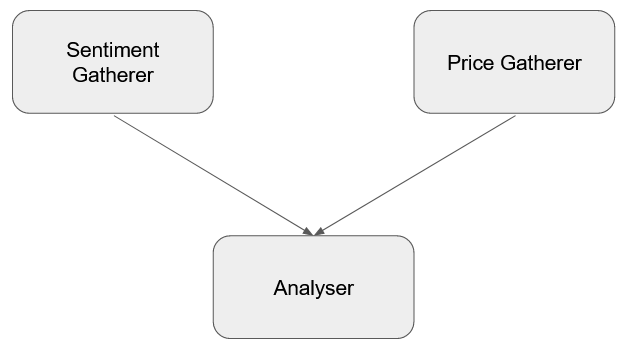
\includegraphics[width=15cm,height=5cm,keepaspectratio]{design/OverallStructure.png}
    \caption{Overall Structure}
    \label{fig:overallstructure}
\end{figure}

\subsection{The Price Gatherer}

The Price Gatherer's purpose is to build a timeline of prices for a given company. It takes in data-points in reference to a given company's prices ordered by date and filters them in order to adapt them to the system. It can be broken down into 3 stages, arranged as seen in figure \ref{fig:pricegathererstructure}:
\begin{itemize}
    \item \texttt{The Price Source} -- Handles the gathering of price values
    \item \texttt{Key Filtering} -- Filters the raw data and extracts the desired keys for each data-point
    \item \texttt{The Return Adder} -- Adds returns to the data-points as extra keys
\end{itemize}

The overall output of this section is an array of JSON objects, ordered by the date key. Each of these objects containing the keys, the exception being the return keys as will be discussed:
\begin{itemize}
    \item \texttt{date} -- the date of the data-point
    \item \texttt{close} -- the closing price for the date of the data-point
    \item \texttt{symbol} -- the symbol representing the company this data is about
    \item \texttt{volume} -- the volume of trades for the date of the data-point
    \item \texttt{return1Day} -- the return in relation to 1 data-point previous
    \item \texttt{return7Day} -- the return in relation to 7 data-points previous
    \item \texttt{return14Day} -- the return in relation to 14 data-points previous
    \item \texttt{return21Day} -- the return in relation to 21 data-points previous
\end{itemize}

\begin{figure}[h]
    \centering
    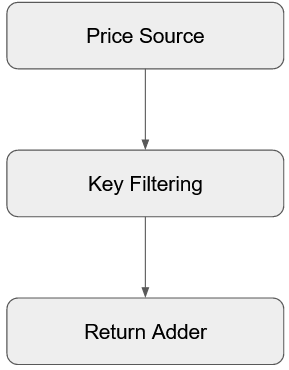
\includegraphics[width=15cm,height=5cm,keepaspectratio]{design/PriceGathererStructure.png}
    \caption{Price Gatherer Structure}
    \label{fig:pricegathererstructure}
\end{figure}

\paragraph{The Price Source}

The purpose of the price source component is to contact the IEX Cloud API and collect daily price points for a given period. Due to the limitations of the tier chosen with the platform, the maximum period allowed is the past 5 years.

\paragraph{Key Filtering}

The IEX Cloud API returns an array of JSON objects, ordered by date, with each object containing the date, close, symbol and volume keys, as well as many others. This component filters out only the desired keys, removing the ones that are not required within the system. This allows the data to managed more easily, as well as any processes being executed faster, and anything that is stored requires less memory. This thus simplifies the process. However, it does create room for future expansion and potential improvement in understanding, as more specificity would be added.

\paragraph{The Return Adder}

The keys missing after the key filtering are those that determine the return values. This component adds them to each entry. The return for a given n determines the difference in closing prices between the current entry and the entry n days before. The returns require previous entries, therefore the first n entries will not have a return given n, the number of previous entries required. The reasoning for adding returns is due to the fact that it allows to examine the change between days rather than the full days themselves, since this project is studying the change in market values.

\subsection{The Sentiment Gatherer}

The Sentiment Gatherer's purpose is to build a timeline of sentiment for a given company. It takes in articles and a dictionary and processes them together in order to create an array of sentiment values ordered by date. It can be broken down into 6 stages, arranged as seen in figure \ref{fig:sentimentgathererstructure}:
\begin{itemize}
    \item \texttt{The Article Source} -- Handles the gathering of articles
    \item \texttt{The Article Parser} -- Parses the raw articles into a format usable by the system
    \item \texttt{The Dictionary} -- Handles the extraction of the dictionary from it's source
    \item \texttt{Key Filtering} -- Filters the dictionary entries and extracts only the desired keys
    \item \texttt{The Sentiment Extractor} -- Uses the dictionary entries in order to extract frequencies of sentiment from the articles
    \item \texttt{Z-Scores} -- Modifies the sentiment extracted from absolute values to relative values using z-scores
\end{itemize}

The overall output of this section is an array of JSON objects, ordered by the date key. Each of these objects containing the keys:
\begin{itemize}
    \item \texttt{date} -- date of the data-point
    \item \texttt{articles} -- z-score of number of articles
    \item \texttt{totalWords} -- z-score of number of total words
    \item \texttt{positiveSentiment} -- z-score of number of positive sentiment words
    \item \texttt{negativeSentiment} -- z-score of number of negative sentiment words
\end{itemize}
The reasoning for using z-scores is due to the fact that it allows to examine the change between days rather than the full days themselves, since this project is studying the change in market values.

\begin{figure}[h]
    \centering
    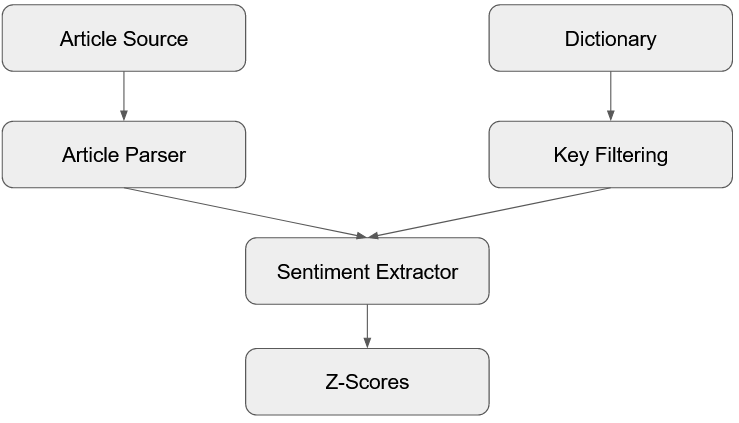
\includegraphics[width=15cm,height=5cm,keepaspectratio]{design/SentimentGathererStructure.png}
    \caption{Sentiment Gatherer Structure}
    \label{fig:sentimentgathererstructure}
\end{figure}

\paragraph{The Article Source}

The purpose of the article source is to provide the articles that will be used in the system.

\paragraph{The Article Parser}

The purpose of this component is to import the files and parse them into a format usable by the system, this being JSON. This is required for LexisNexis as the articles downloaded have the rich text format. The output of this component returns an array of JSON objects, this allows metadata to be stored alongside the body of the article itself.

\paragraph{The Dictionary}

The purpose of this component is to handle the extraction of the dictionary into a JSON object array from the excel sheet it is stored in.

\paragraph{Key Filtering}

The purpose of this component is to filter only the desired keys from the dictionary, in order to decrease processing times and memory requirements. This quite importantly simplifies the analysis significantly. However, it does create room for future expansion and potential improvement in understanding, as more specificity would be added.

\paragraph{The Sentiment Extractor}

The purpose of the component is to extract sentiment frequencies from the articles, using the dictionary as a reference. What this means is that it tallies the number of words belonging to each desired attribute for each article. The articles are then joined by date, tallied appropriately, and ordered by date. The output is an array of JSON objects which represent the absolute values of the different attributes required.

\paragraph{Z-Scores}

The purpose of the component is to take the JSON object produced from the previous component and get the z-scores of the number of articles, of the total number of words in relation to the number of articles, and of each of the sentiment attributes in relation to the total number of words.

\subsection{The Analyser}

There are three components that are predecessors of the main analyser components. These are:
\begin{itemize}
    \item \texttt{The User Interface} -- A command line menu was created in order to organise and utilise all of the various components in a fast and easy way
    \item \texttt{The Joiner} -- It joins the sentiment and prices data-sets where they overlap. Creating two new data-sets.
    \item \texttt{The Period Selector} -- This allows for different periods to be explored within the dataset
\end{itemize}

The Analyser's purpose is to take the timelines produced by the Price Gatherer and the Sentiment Gatherer and analyse them in various different ways. It is a set of unrelated components which allow for the full analysis required in order to understand the data in the way desired for this project. The sub-components build for this component are the following:
\begin{itemize}
    \item \texttt{Return Vs Sentiment Grapher} -- Allows the graphing of sentiment keys and price keys in a time-series
    \item \texttt{Single Point Estimator} -- Uses machine learning model to estimate next day returns
    \item \texttt{Autocorrelator} -- Calculates correlation of key with itself with given lag
    \item \texttt{Return Vs Sentiment Correlator} -- Calculates correlation of given keys with predefined lags
    \item \texttt{Descriptive Statistics} -- Calculates and displays descriptive statistics of given key
    \item \texttt{Vector Autoregressor} -- Calculate Vector Autoregression elements
\end{itemize}

\paragraph{The User Interface}

This is an essential part for the usability of the system create. It allows a user to navigate through the system, and analyse the data in any desired way, given the constraints of the system. It is a set of menu's which allow the selection of any given component and the selected that is desired in the analysis.

\paragraph{The Joiner}

For certain parts of the analysis the data being analysed should be overlapping appropriately. This is an important feature as the price and sentiment data-set have different start and end dates. As well as this not all dates that are covered by one are covered by the other, therefore data must be inserted in these cases, with the assumption that there was no activity for the data that did not exist previously. This has two main cases the first being a day with not sentiment, the assumption can be made that the day has zero sentiment, allowing an appropriate object to be inserted. As for days with no price the assumption can be made that the prices did not vary and the return was 0. However, this case is rare, and no examples of such a situation have been seen.

\paragraph{The Period Selector}

The purpose of this component is quite straight forward. It allows for the narrowing of scope. This is done by allowing for the selection of subsets of the main datasets by selecting a shorted period to examine.

\paragraph{Return Vs Sentiment Grapher}

The purpose of this component is to allow the creation of graphs which compare various columns between the prices data-set and the sentiment data-set. It however also allows the graphing of multiple columns in the one data-set, as well as graphing columns from only one data-set. This allows the creation of any graph desired. The graphs are graphed against the date of the data-point.

\paragraph{Single Point Estimator}

The purpose of this component is to explore the applications of machine learning models in this area. The models take in data from a given date, this being sentiment and price data and estimate whether the nest day would have a positive or negative return. This allows for the comparison between machine learning methods and mathematical methods. The output of this component is two fold. The first item returned is the accuracy of the most accurate model. The second item returned is said model, thus allowing for potential future use and/or storage. This area could be explored in a lot more depth through the use of a more substantial amount of models, hyperparameters and the like.

\paragraph{Autocorrelator}

The autocorrelator allows for the calculation of the correlation of a given column in a given data-set with itself, and it displays the information with n days of lag, where n is selected by the user. This is to help understand how closely related the data is with itself in nearby days, allowing for insight into whether there is a possibility of this data affecting itself. It is important to note, however, that high values of correlation only indicate that there is a potential relationship between days, and does not indicate necessarily causation.

\paragraph{Return Vs Sentiment Correlator}

The return vs sentiment correlator allows for the calculation of three kind of correlation. These are correlation between negative sentiment and 1 day return on the same day, the correlation between these when 1 day return is one day after the negative sentiment, and the correlation between these when negative sentiment is one day after the 1 day return. An expansion to this component would be to allow for different amount of lag between these data-sets. Similarly to the autocorrelator it is important to note, however, that high values of correlation only indicate that there is a potential relationship between elements, and does not indicate necessarily causation.

\paragraph{Descriptive Statistics}

The purpose of the component is to gather a column from the data-set and explore it's descriptive statistics, in order to understand said column better. On top of the descriptive statistics, this component prints out a graph which allows for a visual element. This can be of great aid when trying to understand the significance of the descriptive statistics.

\paragraph{Vector Autoregressor}

The purpose of this component is to explore causation between return and negative sentiment column using vector auto-regression. This adds a layer of rigorousness to the previously explored correlations, as it allows for the understanding of not just what is correlated but which columns cause data in other columns to change. This removes elements such as coincidence.

\section{Scope of Project}

The scope of the project was mainly limited by the data being explored. Many columns were removed from the various data-sources in order to simplify this. The data-set being explored is therefore limited it a general analysis. This can be seen through the use of the generic sentiment columns as well as the basic price columns. On top of this only a certain amount of depth was explored with the machine learning models, correlation and causation. For these reasons I believe there is very large amount of potential expansion to the project, and therefore the understand of the data and its relationships.

\section{Design Summary}

This chapter provides a brief overview of the project, the system design, the handling of the required data and its sources, user interaction with the system, it's design architecture, an explanation of the system components and the scope of the project.